% THIS TEMPLATE IS A WORK IN PROGRESS

\documentclass{article}

\usepackage{hyperref}
\usepackage{fancyhdr}
\usepackage{amsfonts,amsmath}
\usepackage{latexsym}
\usepackage{fullpage}
\usepackage{graphicx}
\usepackage{tikz}
\usepackage{enumitem}
\usepackage{amsthm}
\usepackage{makecell}
\usepackage{graphicx}

%\lhead{\includegraphics[width=0.2\textwidth]{nyush-logo.pdf}}
\fancypagestyle{firstpage}{%
  \lhead{NYU Shanghai}
  \rhead{
  %%%% COMMENT OUT / UNCOMMENT THE LINES BELOW TO FIT WITH YOUR MAJOR(S)
  %\&
  %Data
   Machine Learning 2021}
}

%%%% PROJECT TITLE
\title{Machine Learning Approach to Soccer Player's Overall Rating Prediction}

%%%% NAMES OF ALL THE STUDENTS INVOLVED (first-name last-name)
\author{\href{mailto:ao2186@nyu.edu}{Antai Ouyang \#1}, \href{mailto:xl3215@nyu.edu}{Xianglong Li \#2}, \href{mailto:hl4151@nyu.edu}{Haochen Li \#3}}

\date{\vspace{-5ex}} %NO DATE


\begin{document}
\maketitle
\thispagestyle{firstpage}


\begin{abstract}
    
    
    For this project, we are positioning ourselves as a scouting agency that uses analytics to, among other things, enhance the discovery of talents and help soccer clubs better understand the dynamics (features) that come into play when determining the overall ability of a player. 
    
    Although the $overall$ rating is the most important value either in the real football market or FIFA games, the official rating criteria are still not published. Our model is to predict the $overall$ rating of players given their several capability values. Specially, we will divide players' positions into 4 categories: forwards/strikers, midfielders, backfielders, and goalkeepers, and we will predict overall ratings for each of these categories respectively.
    
    To demonstrate the benefits of our model, we built various charts and evaluated them. In our experiments, we evaluate the performance of 5 different models, which are Linear Regression, Random Forest, Gradient Boosted, K-Nearest Neighbors, and Neural Network. Finally, we choose the best model and the most useful model among all these models and discussed their different usages.
    
\end{abstract}


\section*{Introduction}
The Fédération Internationale de Football Association (FIFA) publishes the overall rating and other metrics for soccer players every year in its authorized soccer game. Intuitively, the metrics of a player can affect the overall rating of a player. However, the exact rating criteria are still not published. Data analysis on soccer players' performance and abilities are being more and more valued by current soccer clubs. Thus, our project aims to predict the overall rating of players given their capability values.

Several data analyses projects have been designed for this dataset. However, these projects only focus on evaluating the metrics of players but failed to predict
the overall rating of players. Some projects tried to predict the overall rating of players, but these projects still lack the comparison among different models
to choose the best one or give any persuasive insights or conclusions. Our project tries different models for rating prediction and determines their performances to find the best model and give insightful conclusions and opinions.

We will implement regression methods in machine learning to this problem. We plan to train our model based on a set of training data randomly selected from our dataset, and then test our model on a stand-out test set also selected from our dataset. In this way, we can create and validate a model predicting the overall rating of a player.


Our project dataset is FIFA 2019 players attribute dataset, which is collected from Kaggle. This dataset includes 89 attributes of a soccer player, and our project only uses some of these attributes concerning only player capability. Details of data processing will be deeply illustrated in the Dataset chapter.

We will implement linear regression and neural networks in our project. The solution chapter gives the details of our models, including their hyperparameters. To finish this model fitting and predicting process, we plan to randomly select data from our dataset, and then split the selected data into training and testing sets to implement cross-validation.

We will evaluate and compare the performance of these 2 models based on their $r2 score$ and testing $RMSE$. Besides, we will inspect the difference between these 2 models in practical use, and will mainly evaluate the usefulness of parameters of linear regression. This part will be further discussed in the Results and Discussion chapter.


\section*{Dataset}

\subsection*{Dateset overall}

Our project dataset is FIFA 2019 players attribute dataset, which is collected
from Kaggle. This dataset includes 89 attributes of a soccer player, and our
project only uses some of these attributes concerning only player capability.
Besides, considering that goalkeepers have a different set of capability
metrics compared with other players, we will only consider data records of nongoalkeepers in our model.



\subsection*{Data processing}

Now we beginning the data processing.
There are 18206 players for which 89 features each are provided. Firstly, we should drop the duplicate entries. 
Then we check the columns (attributes). These columns can be grouped into 6 categories as follows: 

\begin{table}[htpb]
    \centering
    \begin{tabular}{|l|l|}
    \hline
    \makecell[c]{\textit{Category}}     &       \makecell[c]{\textit{Attributes}} \\ \hline
    \textit{Basic Information}          &       \makecell[c]{\textit{ID, Name, Age, Photo, Nationality, Real Face, Height, Weight,} \\
                                                \textit{Body Type, Special, Flag, Position, Club, Club Logo, Work Rate,} \\
                                                \textit{Jersey Number, Weak Foot, Preferred Foot, Skill Moves, Reputation}} \\ \hline
    \textit{Ratings}                    &       \makecell[c]{\textit{Overall, Potential, LS, ST, RS, LW, LF, CF, RF, RW, LAM,} \\
                                                \textit{CAM, RAM, LM, LCM, CM, RCM, RM, LWB, LDM, CDM,} \\
                                                \textit{RDM, RWB, LB, LCB, CB, RCB, RB}} \\ \hline
    \textit{Market Value Related}       &       \makecell[c]{\textit{Value, Wage, Joined, Loaned From, Contract Valid Until, Release Clause}} \\ \hline
    \textit{Abilities}                  &       \makecell[c]{\textit{Crossing, Finishing, HeadingAccuracy, ShortPassing, Volleys, Dribbling,} \\
                                                \textit{Curve,FKAccuracy, LongPassing, BallControl, Acceleration, SprintSpeed,} \\
                                                \textit{Agility, Reactions, Balance, ShotPower, Jumping, Stamina, Strength,} \\
                                                \textit{LongShots, Aggression, Interceptions, Positioning, Vision, Penalties,} \\
                                                \textit{Composure, Marking, StandingTackle, SlidingTackle}} \\ \hline
    \textit{Goalkeeper Abilities}       &       \makecell[c]{\textit{GKDiving, GKHandling, GKKicking, GKPositioning, GKReflexes}} \\ \hline
    \end{tabular}
    \caption{Columns (attributes) in the original dataset.}
\end{table}

\par Our model only focuses on predicting the overall rating of a player. Thus, we only need to keep those attributes related to the ability of players and drop the other irrelevant attributes. Besides, our model does not consider ratings on different positions for the same player. Thus, we only keep all $Abilities$, all $Goalkeeper\; Abilities$, $Age$ and $Position$ in $Basic\; Information$, and $Overall$ in ratings as our target value.

\par After deleting all the irrelavent attributes, we still have to delete data records with missing values. These records are resulted from the lack of player information of some small clubs, and they could introduce errors into our prediction. The null values in each column are counted and sorted as follows:

\begin{table}[]
\centering
\begin{tabular}{|l|l|l|l|}
\hline
\textit{Index} & \textit{column name}          & \textit{Total missing} & \textit{Percent missing} \\ \hline
\textit{0}     & \textit{Position}             & \textit{60}            & \textit{0.003295}        \\ \hline
\textit{1}     & \textit{GKReflexes}           & \textit{48}            & \textit{0.002636}        \\ \hline
\textit{2}     & \textit{Curve}                & \textit{48}            & \textit{0.002636}        \\ \hline
\textit{3}     & \textit{Agility}              & \textit{48}            & \textit{0.002636}        \\ \hline
\textit{...}   & \textit{...}                  & \textit{...}           & \textit{...}             \\ \hline
\textit{35}    & \textit{Stamina}              & \textit{48}            & \textit{0.002636}        \\ \hline
\textit{36}    & \textit{Overall}              & \textit{0}             & \textit{0.000000}        \\ \hline
\textit{37}    & \textit{Age}                  & \textit{0}             & \textit{0.000000}        \\ \hline
\end{tabular}
\caption{Missing value percent.}
\end{table}

\par By observing these missing values in our dataset, all missing data lies in the 60 records with missing $Position$ value. After deleting these records with missing values, we have 18147 rows left in our dataset. After that, we still should inspect the data types of each column, and this is to ensure the input attributes of our model are all of type $int$ to guarantee that our model works. The only attribute violating this in our model prediction dataset is $Position$. This attribute only indicates the position of a soccer player.
\par We divide all records into different categories according to their positions. In this way, we can get rid of this String-typed attribute. Besides, in the real soccer industry, players can be categorized according to their positions. We mainly divide players into 4 positions: \textbf{Forward}, \textbf{Midfielder}, \textbf{Back}, and \textbf{Goalkeeper}. Besides, for prediction on players on any position, we also keep the original dataset, but only delete its $Position$ column.
\par Finally, we implement data normalization on each column. We use the expression below to calculate normalized data:
$$Normalized = \frac{Original-Mean}{Variance}$$
In which $Mean$ and $Variance$ are the mean and variance of the original data $Original$. After this normalization, we output all 4 categorized datasets and the original dataset into 5 CSV files respectively.

\section*{Solution}
We implement 5 models \textbf{Linear Regression}, \textbf{Random Forest}, \textbf{Gradient Boosted}, \textbf{K-Nearest Neighbors} and \textbf{Neural Network}. Below, we will introduce our workflow.

\subsection*{Feature Engineering}
The process of taking raw data and extracting or creating new features that allow a machine learning model to learn a mapping between these features and the target. This might mean taking transformations of variables, such as we did with the log and square root, or one-hot encoding categorical variables so they can be used in a model. Generally, we think of feature engineering as adding additional features derived from the raw data.
In this project, we take the following steps:
\begin{itemize}
    \item Group similar data(delete positions rating)
    \item Convert object type variables to numerical by label encoding(transform string type to int type)
\end{itemize}



\subsection*{Feature Selection}
 The process of choosing the most relevant features in your data. "Most relevant" can depend on many factors, but it might be something as simple as the highest correlation with the target, or the features with the most variance. In feature selection, we remove features that do not help our model learn the relationship between features and the target. This can help the model generalize better to new data and result in a more interpretable model. Generally, I think of feature selection as subtracting features so we are left with only those that are most important.
In this project, we take the following steps:
\begin{itemize}
    \item Delete missing values
    \item Remove features that do not have a significant effect on the dependent variable or prediction of output by backward elimination.
\end{itemize}


\subsection*{Model}.
We will compare five different machine learning models using the great Scikit-Learn library:
\begin{itemize}
    \item Linear Regression
    \item Random Forest Regression
    \item Gradient Boosting Regression
    \item K-Nearest Neighbors Regression
    \item Neutral Network
\end{itemize}

To compare the models, we are going to be mostly using the Scikit-Learn defaults for the model hyperparameters. Generally, these will perform decently but should be optimized before actually using a model. At first, we just want to determine the baseline performance of each model, and then we can select the best-performing model for further optimization using hyperparameter tuning. The default hyperparameters will get a model up and running, but nearly always should be adjusted using some sort of search to find the best settings for your problem!

\subsection*{Metric:}
\subsubsection*{Root Mean Square Error}
Root Mean Square Error (RMSE) is the standard deviation of the residuals (prediction errors). Residuals are a measure of how far from the regression line data points are; RMSE is a measure of how to spread out these residuals are. In other words, it tells you how concentrated the data is around the line of best fit. Root mean square error is commonly used in climatology, forecasting, and regression analysis to verify experimental results.

\subsubsection*{$R^2$ Score}
The $R^2score$ function computes the coefficient of determination. It represents the proportion of variance (of y) that has been explained by the independent variables in the model. It provides an indication of goodness of fit and therefore a measure of how well unseen samples are likely to be predicted by the model, though the proportion of explained variance.

\begin{figure}[!htb]
	\centering
    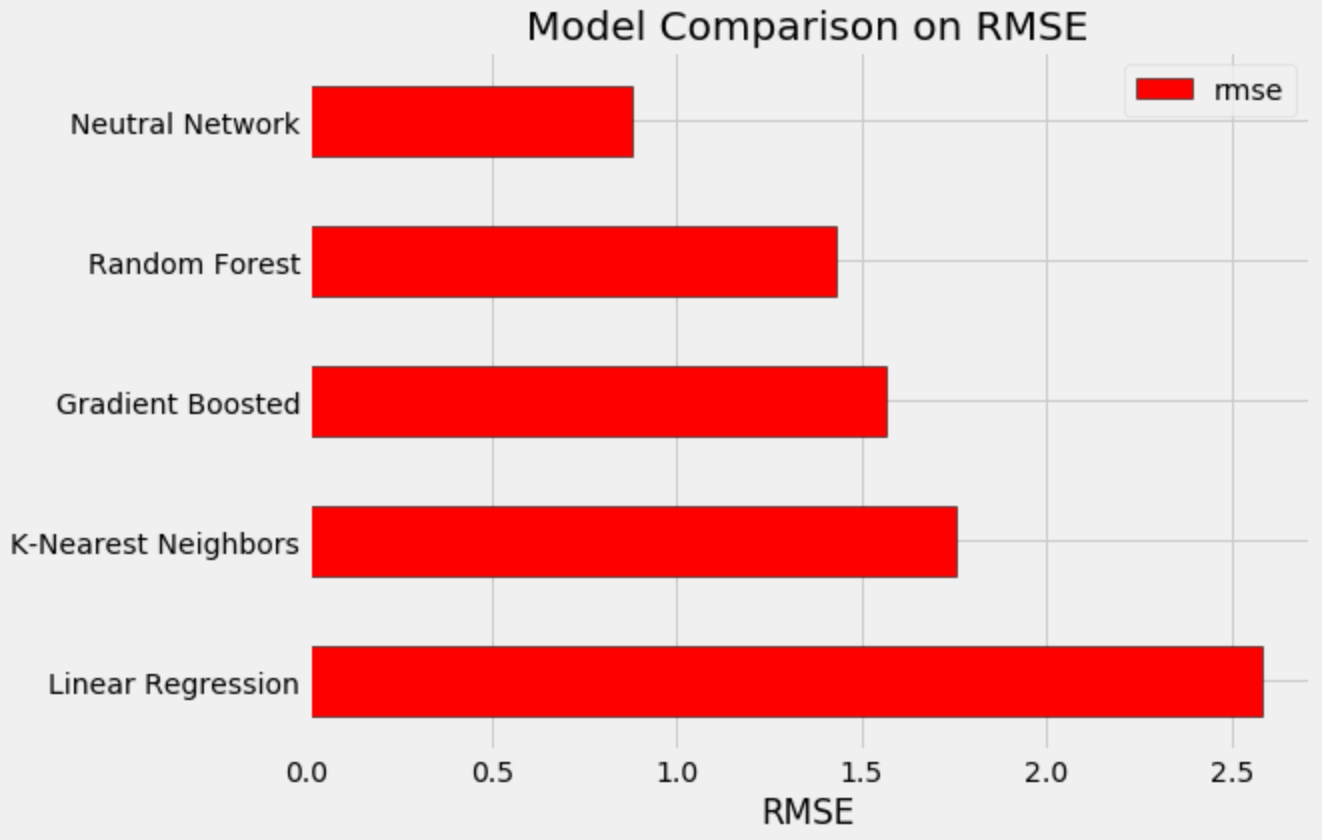
\includegraphics[scale=0.35]{rmse.png}
    \caption{Model Comparison on RMSE}\label{fig1}
\end{figure}

\begin{figure}[!htb]
	\centering
    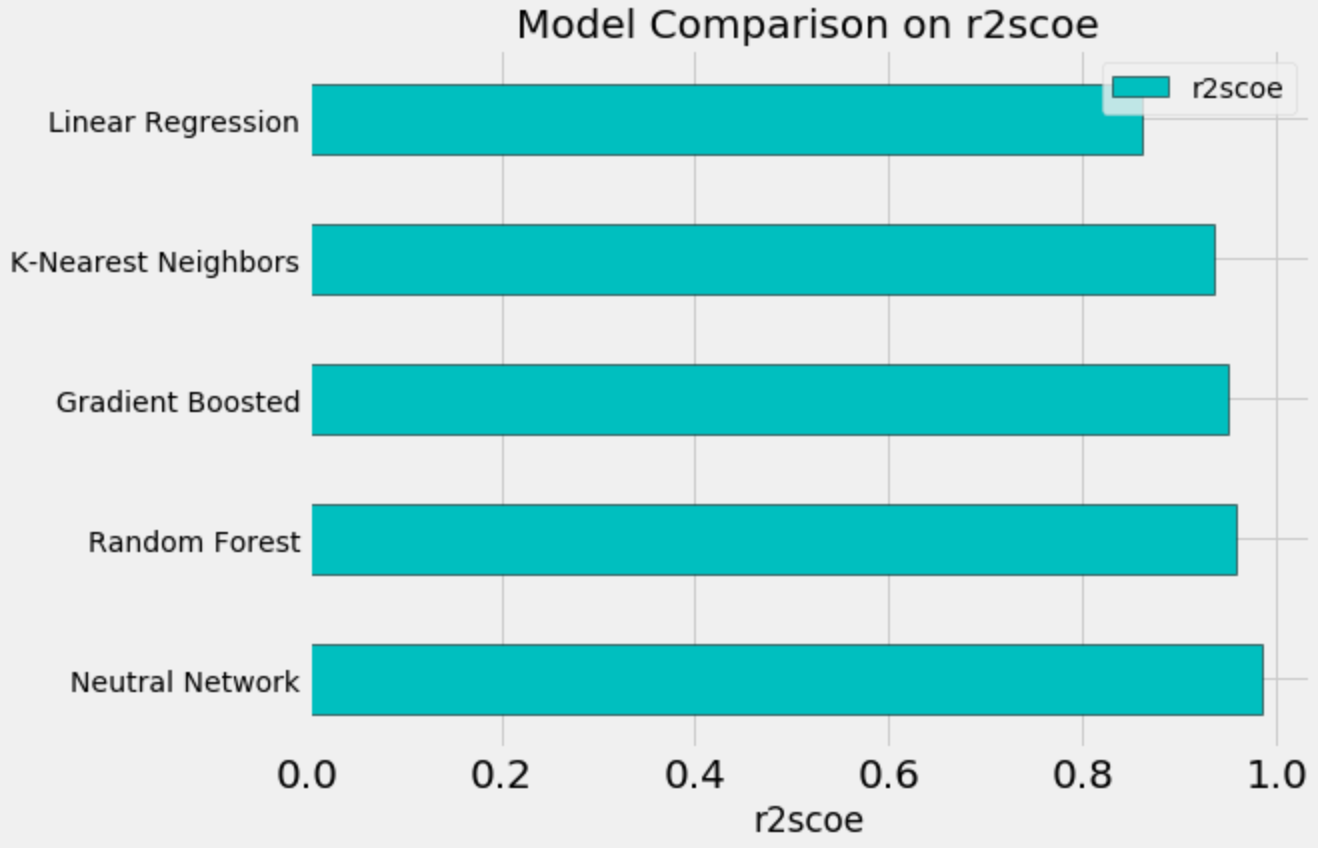
\includegraphics[scale=0.35]{r2score.png}
    \caption{Model Comparison on $R^2$ Score}\label{fig2}
\end{figure}

Figures \ref{fig1} and \ref{fig2} shows our results of running all 5 models mentioned above. Depending on the run (the exact results change slightly each time), the Neutral Network performs the best. We have to admit that this is not the fairest comparison because we are using mostly the default hyperparameters. Nonetheless, from these results, we can conclude that machine learning is applicable because all the models significantly outperform the baseline.
From here, We are going to concentrate on optimizing the best model using hyperparameter tuning. Given the results here, Neural Network has the best performance of all these 5 models. However, considering that only linear regression can give coefficients for each attribute among all these models, linear regression can generate more information and has higher usability than other models. Thus, we will focus on both linear regression and neural networks in the following part.


\subsection*{Model Optimization}
In machine learning, optimizing a model means finding the best set of hyperparameters for a particular problem.

\subsubsection*{Hyperparameters}
First of all, we need to understand what model hyperparameters are in contrast to model parameters :

Model hyperparameters are best thought of as settings for a machine learning algorithm that are tuned by the data scientist before training. Examples would be the number of trees in the random forest or the number of neighbors used in K Nearest Neighbors Regression.

Model parameters are what the model learns during training, such as the weights in the linear regression. We as data scientists control a model by choosing the hyperparameters, and these choices can have a significant effect on the final performance of the model (although usually not as great of an effect as getting more data or engineering features). Tuning the model hyperparameters controls the balance of under vs overfitting in a model. We can try to correct for under-fitting by making a more complex model, such as using more trees in a random forest or more layers in a deep neural network. A model that underfits has high bias and occurs when our model does not have enough capacity (degrees of freedom) to learn the relationship between the features and the target. We can try to correct for overfitting by limiting the complexity of the model and applying regularization. This might mean decreasing the degree of polynomial regression or adding dropout layers to a deep neural network. A model that overfits has high variance and in effect has memorized the training set. Both underfitting and overfitting lead to poor generalization performance on the test set.
The problem with choosing the hyperparameters is that no set will work best across all problems. Therefore, for every new dataset, we have to find the best settings. This can be a time-consuming process, but luckily there are several options for performing this procedure in Scikit-Learn.


\section*{Results and Discussion}
We will use the best model from hyperparameter tuning to make predictions on the testing set and generate our final result. Our model has never seen the test set before, so this performance should be a good indicator of how the model would perform if deployed in the real world.

\begin{figure}[!htb]
	\centering
    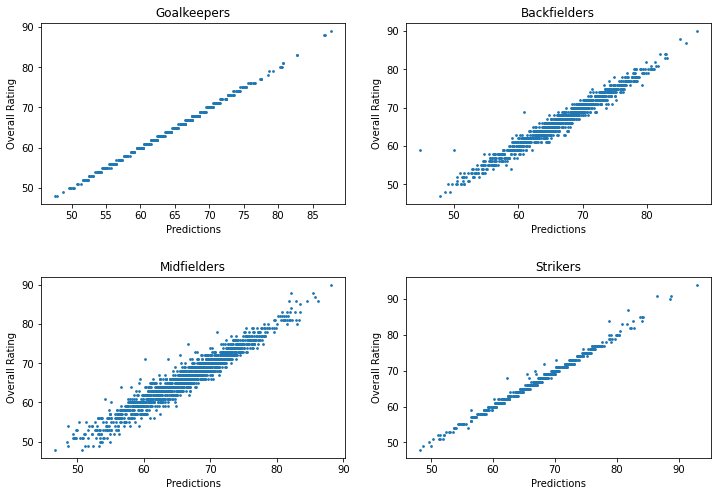
\includegraphics[scale=0.45]{linear.png}
    \caption{Results of linear regression for overall rating prediction.}\label{fig3}
\end{figure}

\begin{figure}[!htb]
	\centering
    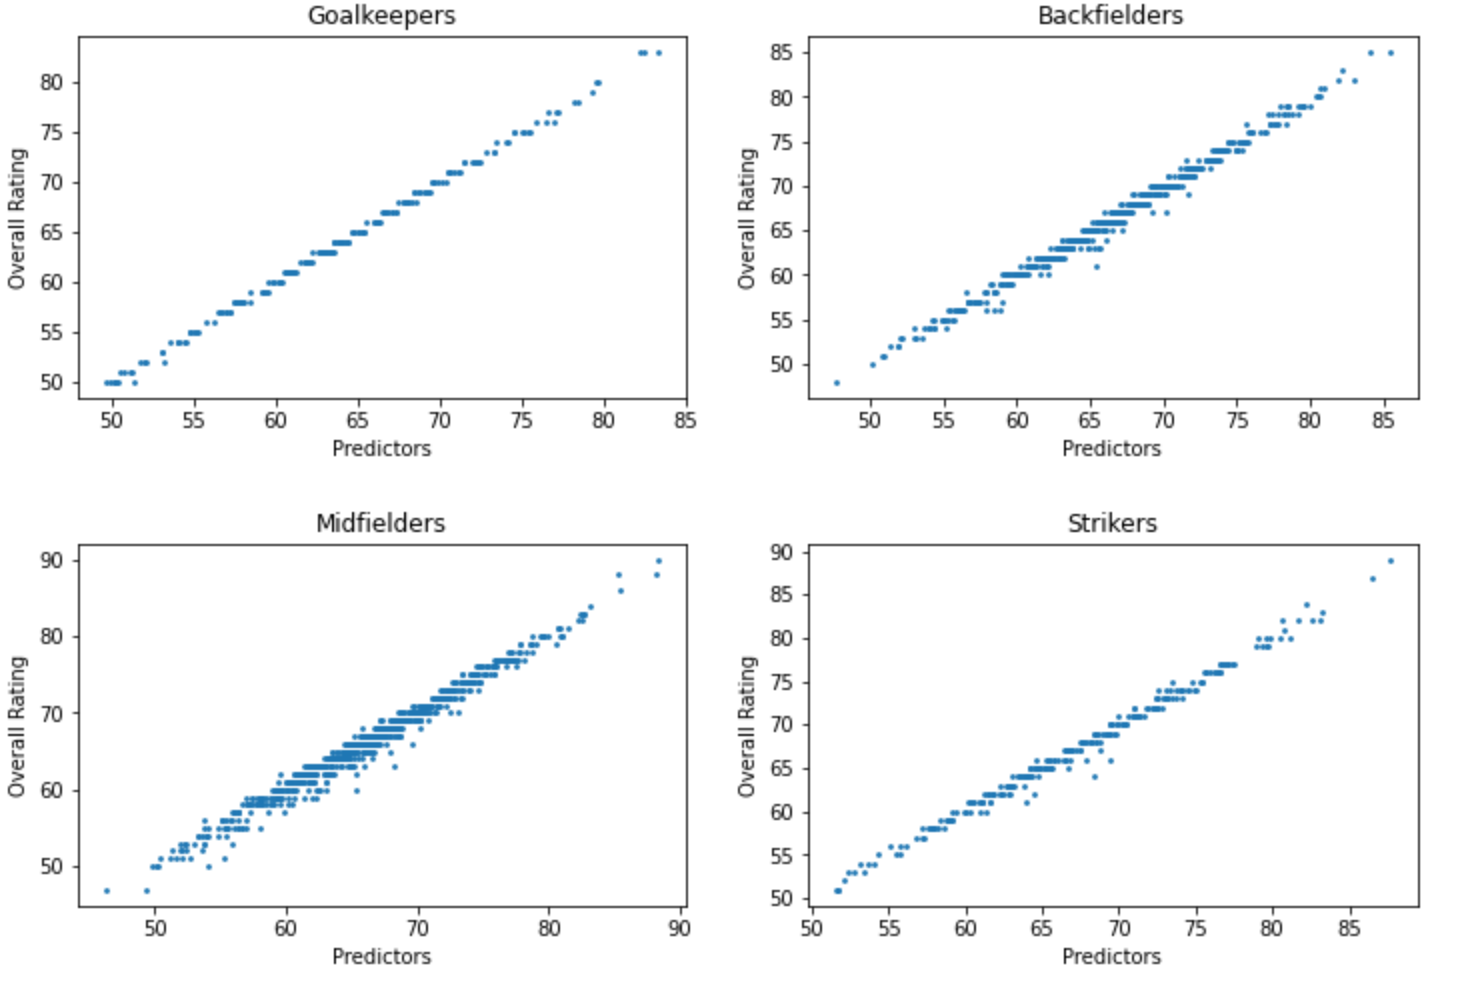
\includegraphics[scale=0.45]{nn.png}
    \caption{Results of neutral network for overall rating prediction.}\label{fig4}
\end{figure}

Figures \ref{fig3} and \ref{fig4} show the results of linear regression and neural network on our testing set.

On the Predictions-Overall Rating axis, the testing results are close to $y=x$, which indicates that our prediction results are almost the same as actual values. This shows that our model performs well in predicting the ability of a player given his / her metrics. 

Besides, for our linear regression model, we also plot its coefficients for all 4 position categories. Figure \ref{fig5} shows the coefficients of the linear regression model for players of each position category.

\begin{figure}[!htb]
	\centering
    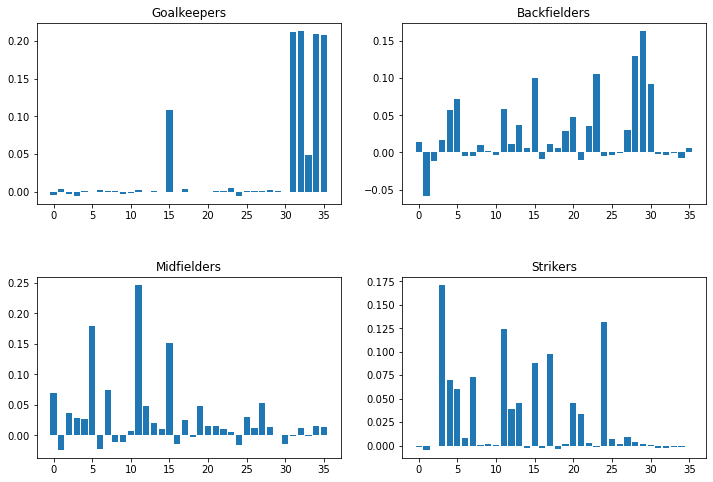
\includegraphics[scale=0.5]{coefs.png}
    \caption{Coefficients of linear regression model.}\label{fig5}
\end{figure}

Investigating these parameters, we have some interesting observations. The value of parameters can reflect the significance of the ability to a position. Below we take midfielders as an example.

We use Python's $heapq$ library to find the 5 largest coefficients and their corresponding attribute names of the linear regression model for midfielders. The results are shown in the table below.

\begin{table}[htpb]
    \centering
    \begin{tabular}{|l|l|}
    \hline
    \textit{Attribute Name}             &       \textit{Coefficient Value} \\ \hline
    \textit{BallControl}                &       \textit{0.24730435} \\ \hline
    \textit{ShortPassing}               &       \textit{0.18084552} \\ \hline
    \textit{Reactions}                  &       \textit{0.14724705} \\ \hline
    \textit{Dribbling}                  &       \textit{0.07184282} \\ \hline
    \textit{Age}                        &       \textit{0.06818059} \\ \hline
    \end{tabular}
    \caption{The 5 largest coefficients and their corresponding attribute names.}
\end{table}

From this table, we can observe that the main attributes contributing to a midfielder's overall rating are ball control, short passing, reactions, and dribbling. This matches the reality since normally a midfielder should control the ball and try to pass it to attacking players nearby. Besides, an older midfielder tends to have a higher overall rating. This also shows that a midfielder with more experience is highly appreciated since $Age$ also has a high coefficient value.

The attributes with high coefficients highly reflect the requirement of the corresponding position. In this way, this information can be quite useful for soccer clubs to design suitable tactics or to improve their training for their own players. A soccer team can even use its own player data to train these coefficients and inspect which attributes reflect the team's style, and then pay more attention to practicing on these aspects in their youth training.

In summary, the neural network model performs a little bit better on accurately predicting overall ratings, while linear regression can provide more information about positions to soccer clubs. From our perspective, these 2 models can be used cooperatively for soccer clubs. The neural network can give an accurate prediction for ratings to find potent players, and linear regression can be used to provide information for helping cultivate young players or planning tactics.

\nocite{*}
\bibliographystyle{IEEEtran}
\bibliography{references}



\end{document}
